\chapter{Resultados}

En este capítulo se van a mostrar resultados obtenidos con las siguientes funcionalidades implementadas: Filtrado, segmentación y documentación.

Para realizar las pruebas se han utilizado la esculturas de Inmaculada Concepción y San Juan Evangelista (Figura \ref{fig:resultados/esculturas}), ambas patrimonio de la Universidad de Granada y cuyos datos DICOM han sido proporcionados por el proyecto de Portal Virtual de Patrimonio de las Universidades Andaluzas, coordinado por la Universidad de Granada.

\begin{figure}[H]
	\centering
	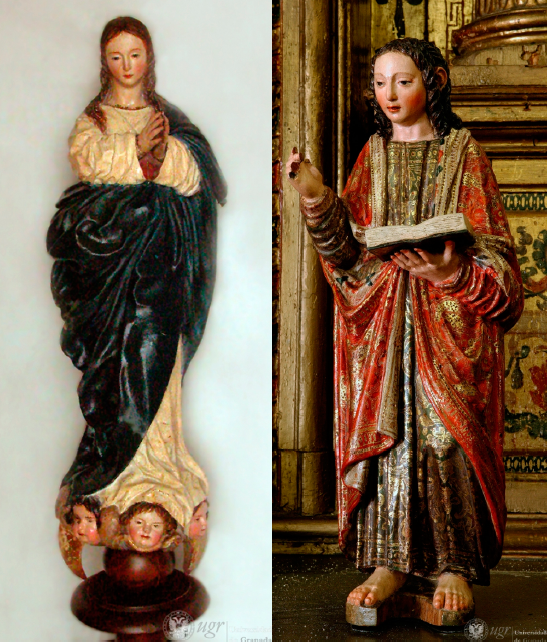
\includegraphics[width=7cm]{imagenes/resultados/esculturas}
	\caption{Esculturas utilizadas para realizar las pruebas. Inmaculada Concepción (izquierda) y San Juan Evangelista (derecha)}
	\label{fig:resultados/esculturas}
\end{figure}

\section{Filtrado}

Se implementaron los filtros de reducción de ruido \textit{gaussiano}, media y mediana dando la posibilidad al usuario a elegir ciertos parámetros.

Para probar estos filtros se ha utilizado la escultura de San Juan Evangelista que es la que más ruido presentaba.

\subsection{Filtro \textit{gaussiano}}

El filtro \textit{gaussiano} es uno de los filtros de suavizado más utilizados. A continuación se va a mostrar los resultados obtenidos con éste para 1, 2 y 3 repeticiones (Figura \ref{fig:resultados/filtrado/gaussiano}).

\begin{figure}[H]
	\centering
	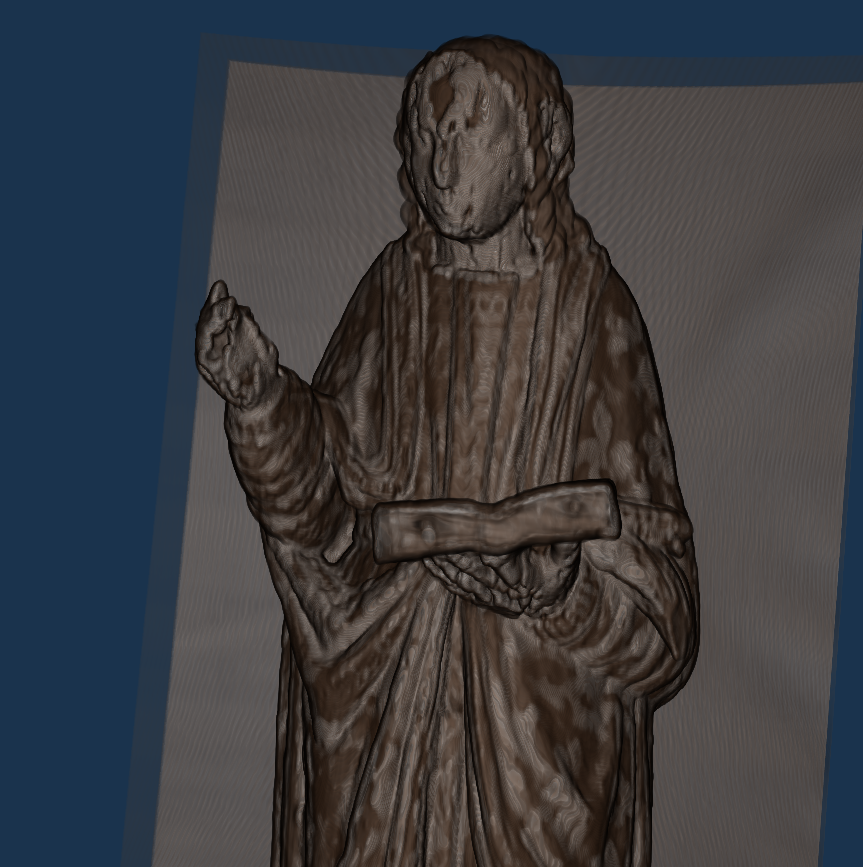
\includegraphics[width=6cm]{imagenes/resultados/filtrado/original}
	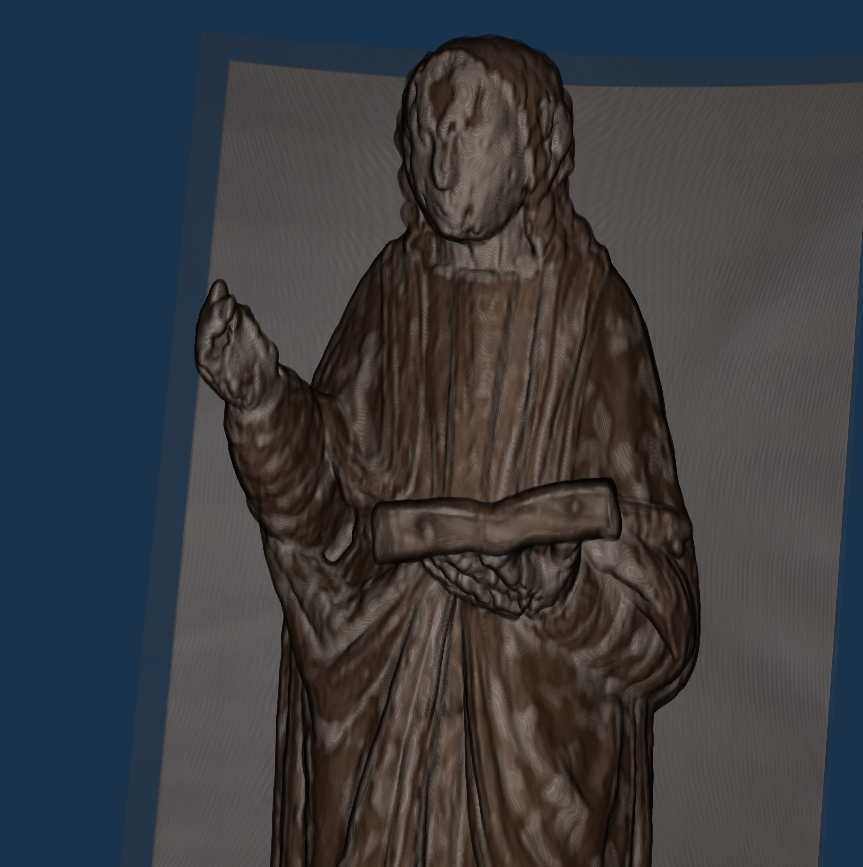
\includegraphics[width=6cm]{imagenes/resultados/filtrado/gaussiano-1}
	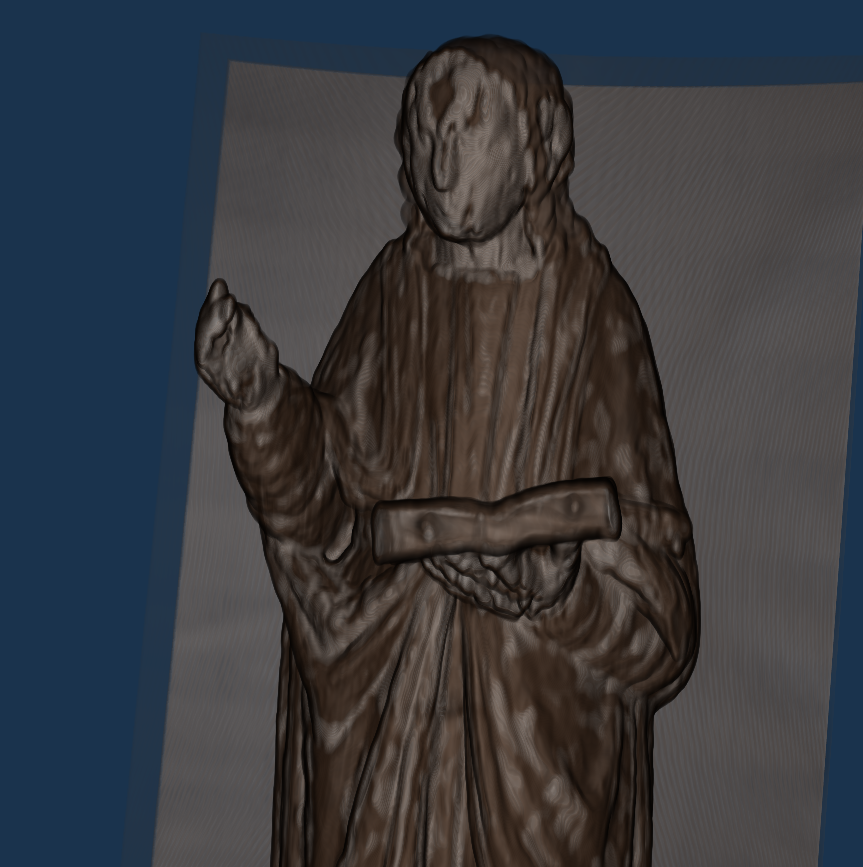
\includegraphics[width=6cm]{imagenes/resultados/filtrado/gaussiano-2}
	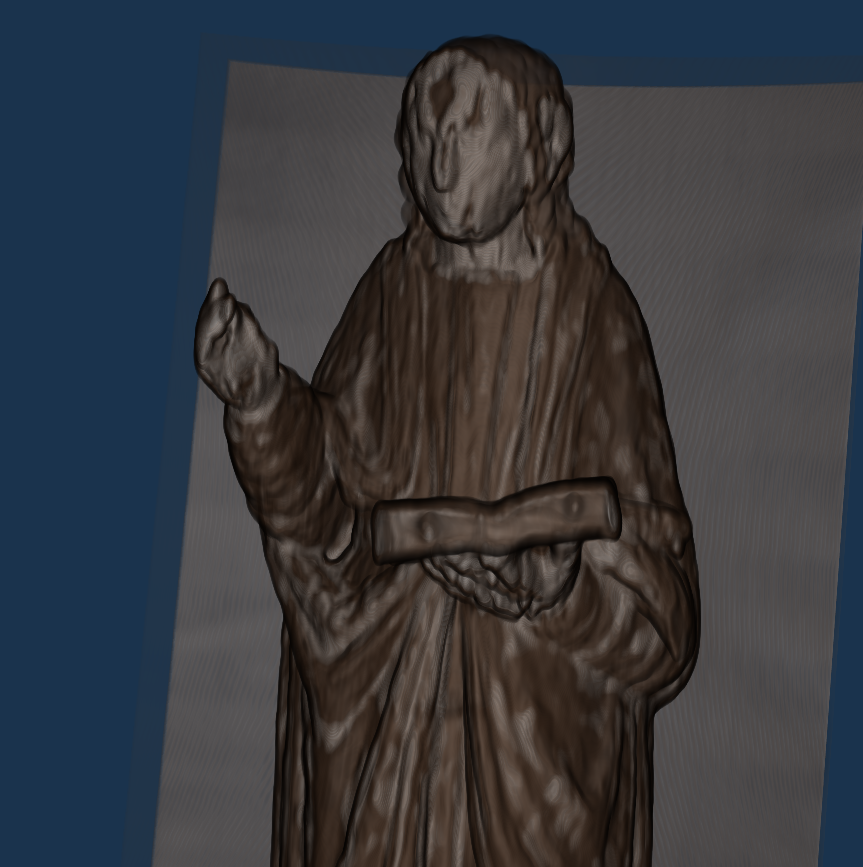
\includegraphics[width=6cm]{imagenes/resultados/filtrado/gaussiano-3}
	\caption{De izquierda a derecha y arriba a abajo: figura original y aplicando el filtro \textit{gaussiano} con 1, 2 y 3 repeticiones}
	\label{fig:resultados/filtrado/gaussiano}
\end{figure}

Se puede observar como apenas hay diferencia entre la original y la que se le ha aplicado el filtro con una sola repetición.

Con la que mejor resultado se obtiene es con la que se le aplica 2 repeticiones, porque con 3 ya empieza a suavizarse de más.

\subsection{Filtro media}

El filtro media es un filtro de suavizado bastante agresivo que usa una convolución y donde el único parámetro que se puede utilizar es el tamaño del vecindario para la convolución. A continuación se va a mostrar los resultados obtenidos con éste para vecindarios de 3x3, 5x5 y 7x7 (Figura \ref{fig:resultados/filtrado/media}).

\begin{figure}[H]
	\centering
	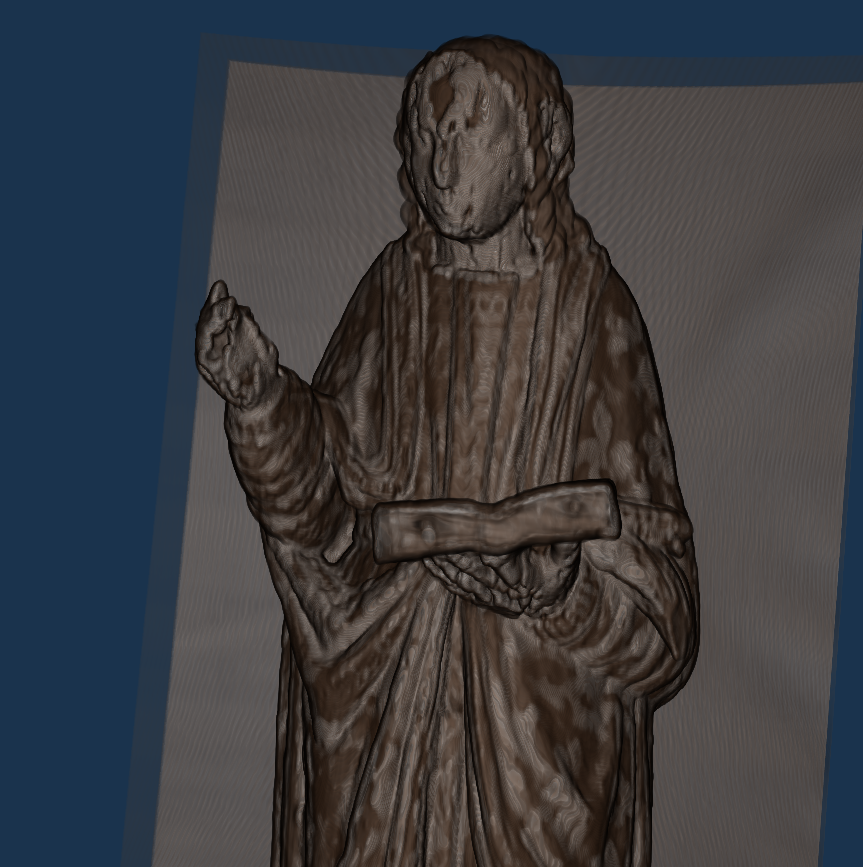
\includegraphics[width=6cm]{imagenes/resultados/filtrado/original}
	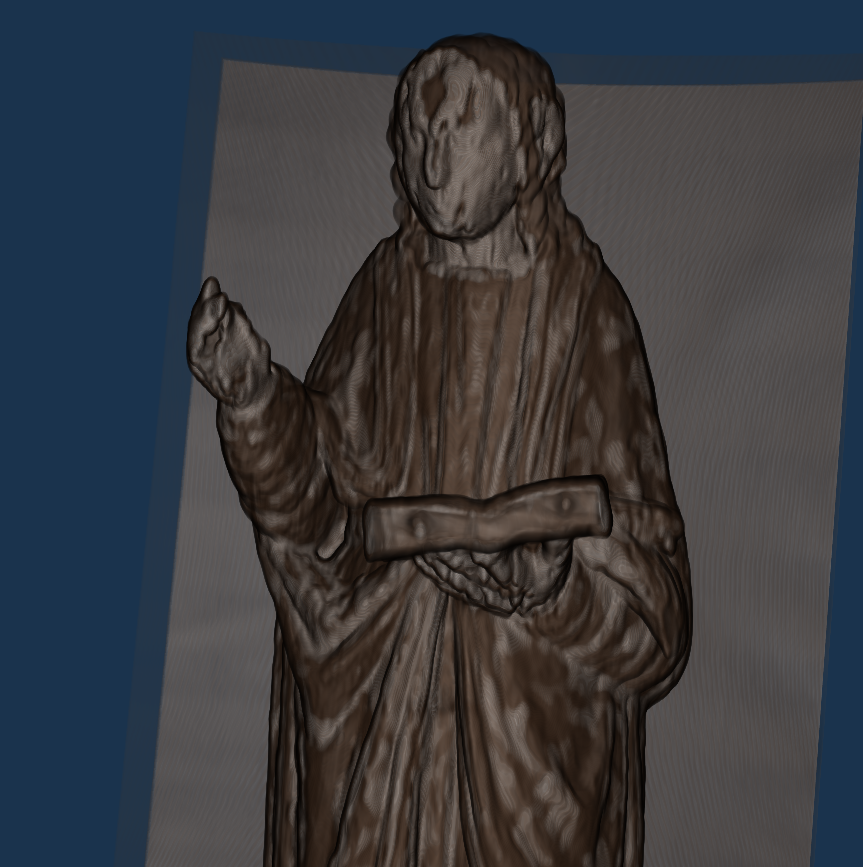
\includegraphics[width=6cm]{imagenes/resultados/filtrado/media-3}
	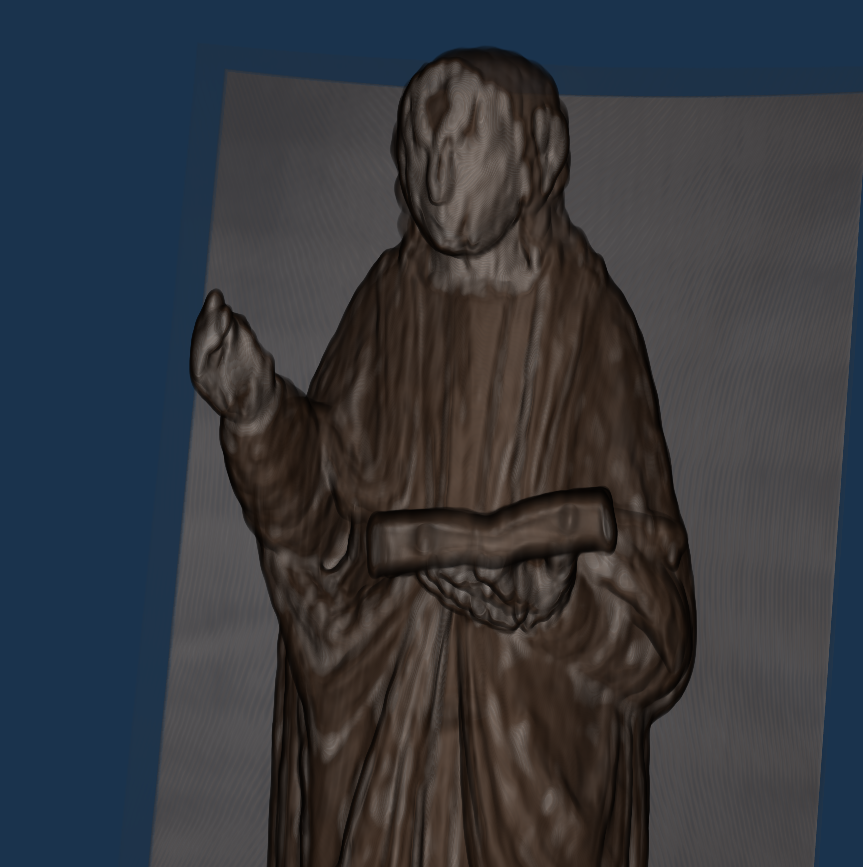
\includegraphics[width=6cm]{imagenes/resultados/filtrado/media-5}
	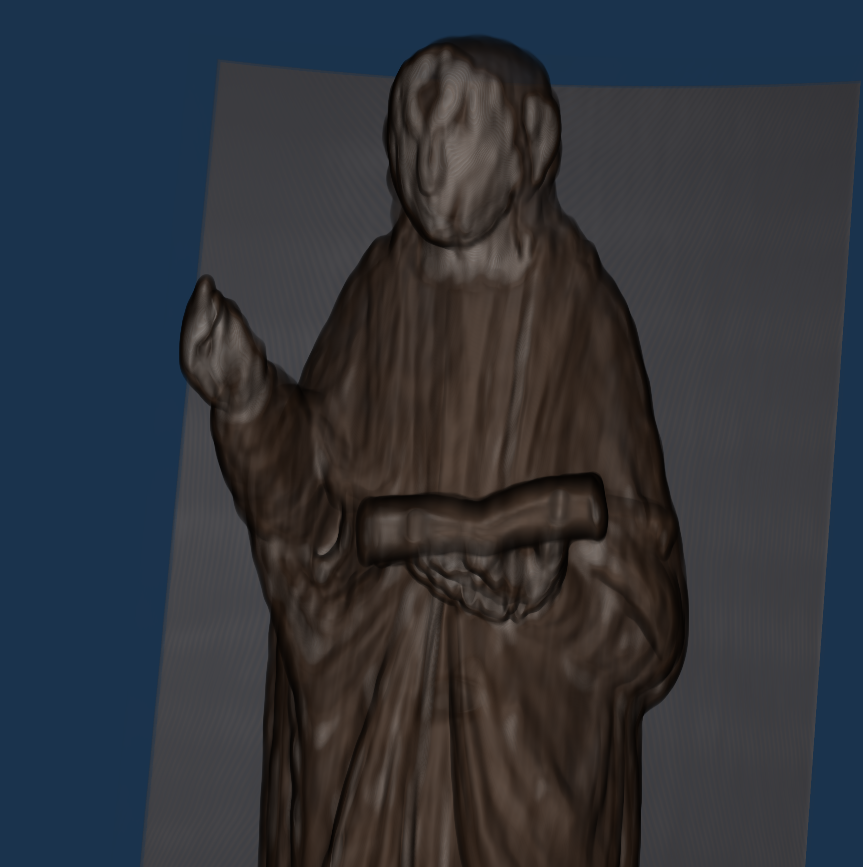
\includegraphics[width=6cm]{imagenes/resultados/filtrado/media-7}
	\caption{De izquierda a derecha y arriba a abajo: figura original y aplicando el filtro media con vecindarios de 3x3, 5x5 y 7x7}
	\label{fig:resultados/filtrado/media}
\end{figure}

Se puede ver como este filtro es bastante más agresivo que el \textit{gaussiano} y se suaviza de más. Por tanto, habría que utilizarlo para imágenes con mucho más ruido.

\subsection{Filtro mediana}

El filtro mediana se utiliza para reducir el ruido de tipo \textit{salt-and-pepper}. Nuestras imágenes no sufren de este tipo de ruido. No obstante se ha probado el filtro con vecindarios de 3x3, 5x5 y 7x7 (Figura \ref{fig:resultados/filtrado/mediana}).

\begin{figure}[H]
	\centering
	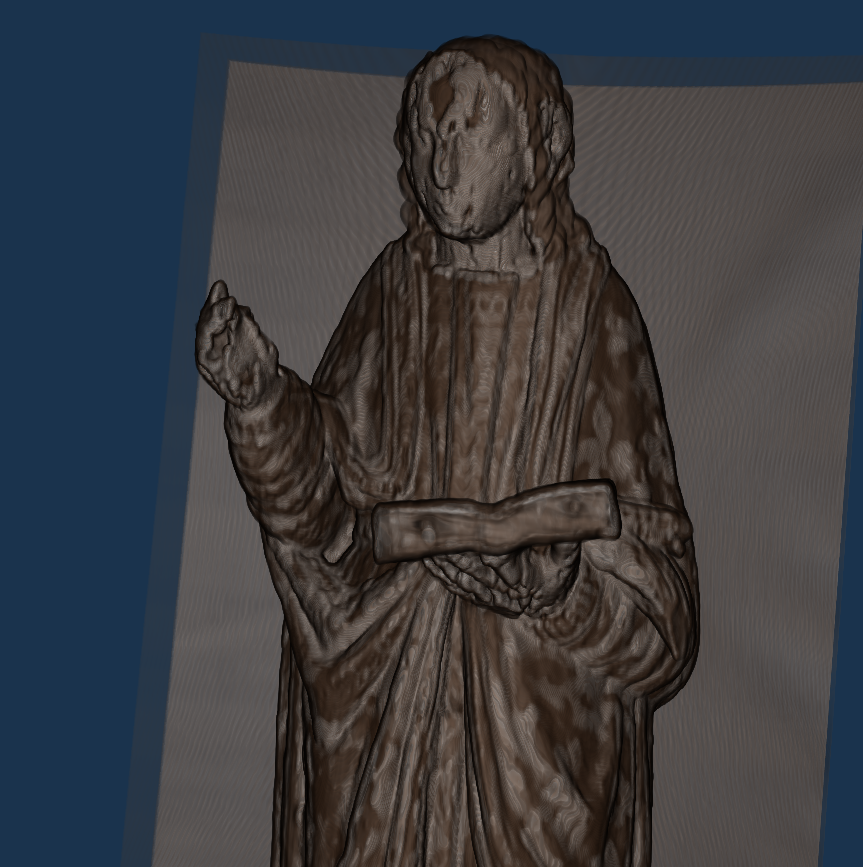
\includegraphics[width=6cm]{imagenes/resultados/filtrado/original}
	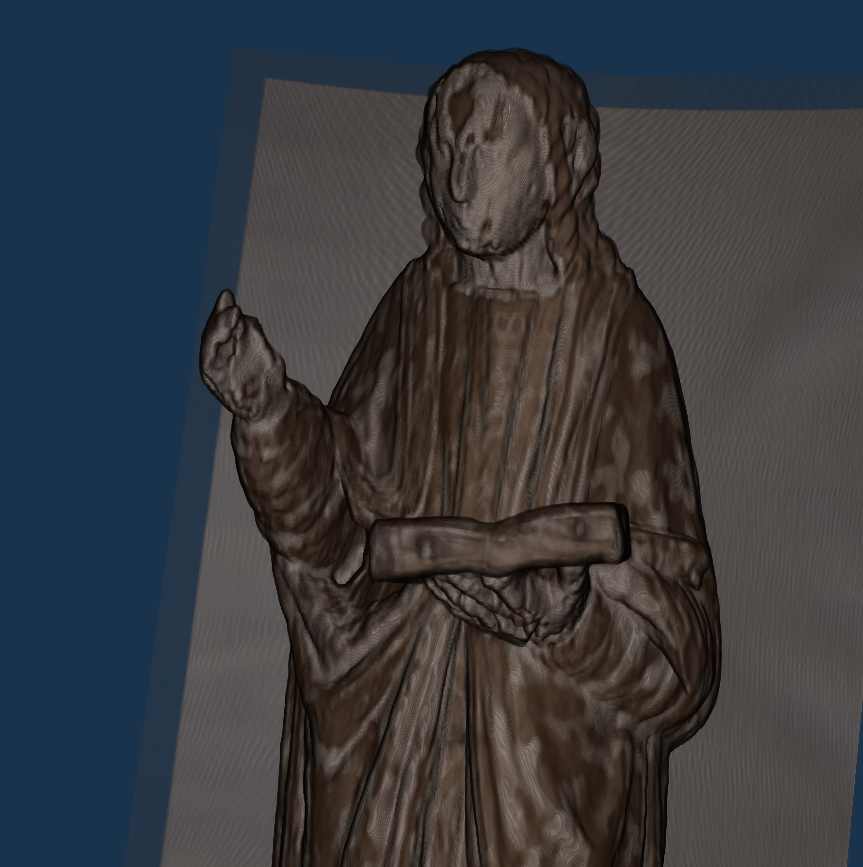
\includegraphics[width=6cm]{imagenes/resultados/filtrado/mediana-3}
	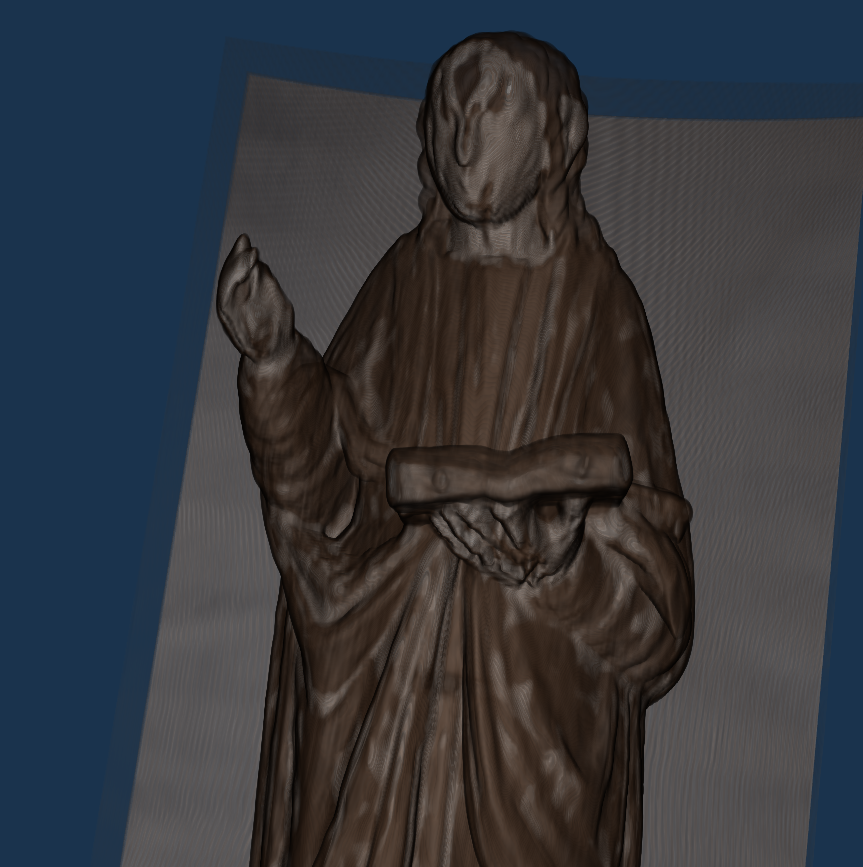
\includegraphics[width=6cm]{imagenes/resultados/filtrado/mediana-5}
	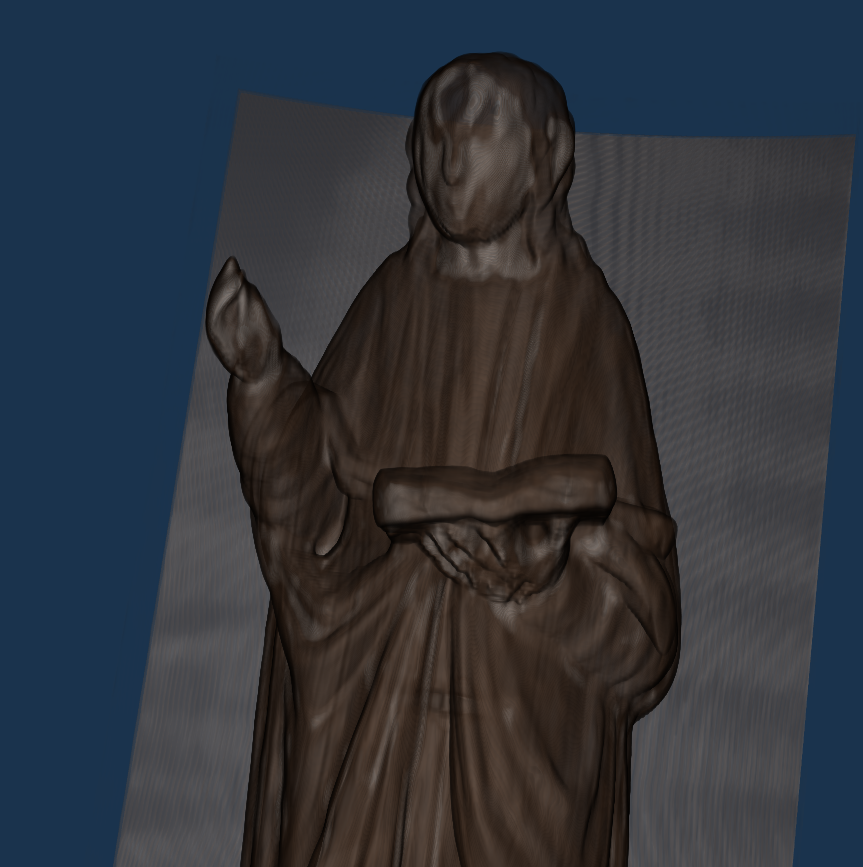
\includegraphics[width=6cm]{imagenes/resultados/filtrado/mediana-7}
	\caption{De izquierda a derecha y arriba a abajo: figura original y aplicando el filtro mediana con vecindarios de 3x3, 5x5 y 7x7}
	\label{fig:resultados/filtrado/mediana}
\end{figure}

Los resultados con este filtro son incluso más agresivos que los obtenidos con el de media. Pero es lógico al ser un filtro creado para reducir un tipo de ruido que no presentan nuestras imágenes.
